\section*{Process Models}
%Providing process models is not enough because the process owner is diffident with any result which he/she is simply provided with. Therefore, he/she wants evidence of the goodness of these models. For this purpose, you should perform alignment-based conformance checking. Using the result of the conformance checker, you should motivate why the chosen models are better that any possible alternative (e.g. because of mediating fitness, precision, generalization and simplicity). For each model, also provide its textual description. 

\subsection*{The model of the application's lifecycle}
%filter on event names
%interactive data heuristic miner
%conformance 
%multi-perspective
For modeling the application lifecycle first the data has been filtered. Just the events beginning with "App\_..." are required. This data set is saved by the name "Filtered App". 


\begin{figure}[h]
\centering
\begin{subfigure}{.49\textwidth}
  \centering
  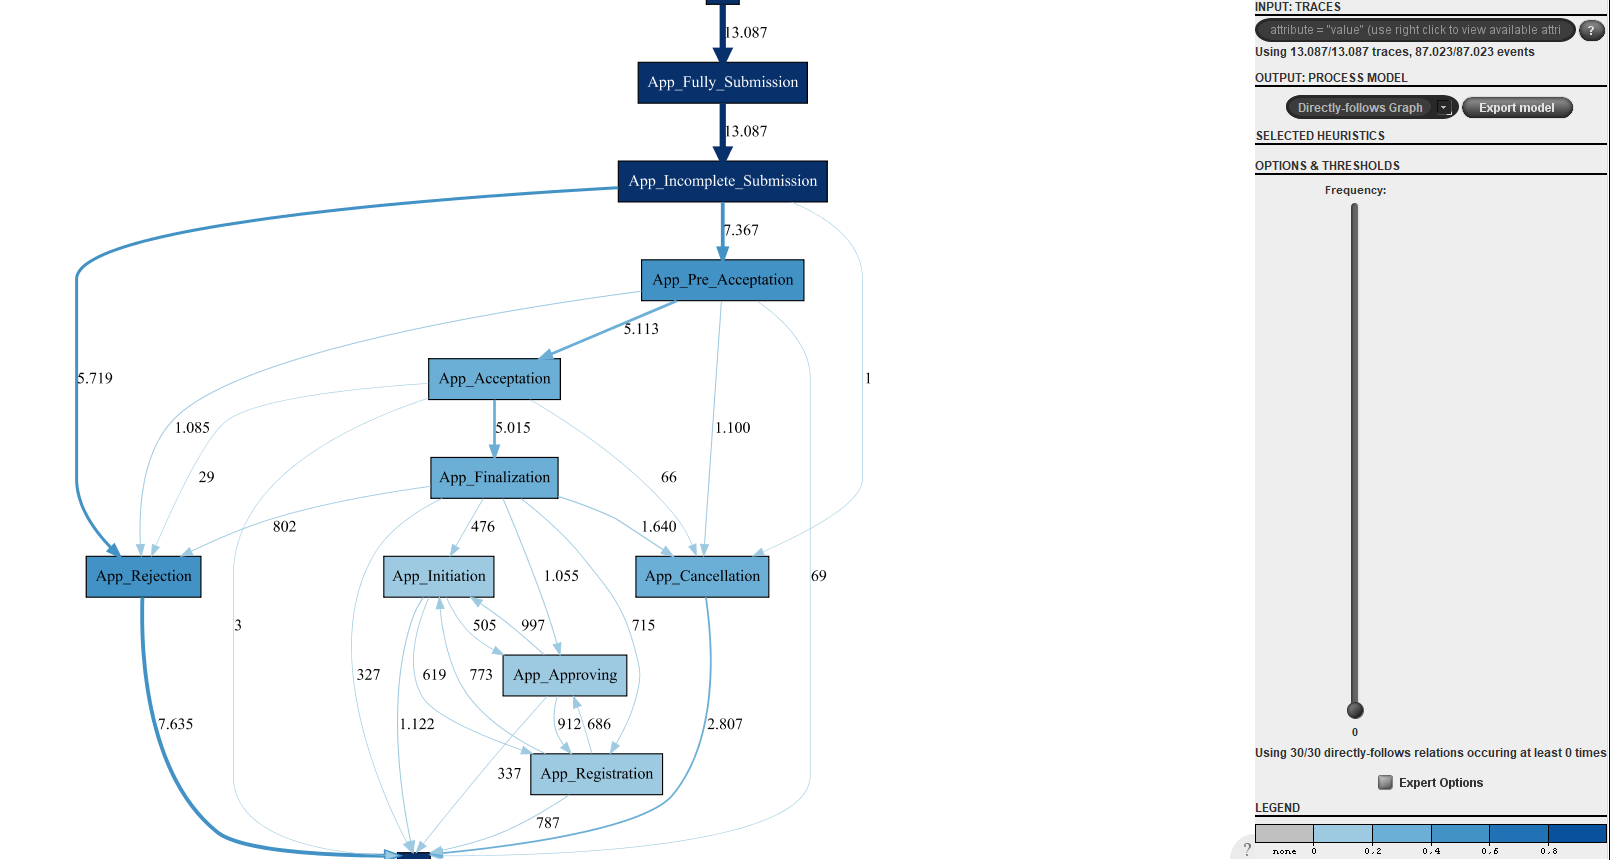
\includegraphics[width=\linewidth]{App_DirectlyFollowedFreq0.PNG}
  \caption{Directly followed graph without frequency filtering}
  \label{fig:APP_DFG0}
\end{subfigure}%
\begin{subfigure}{.49\textwidth}
  \centering
  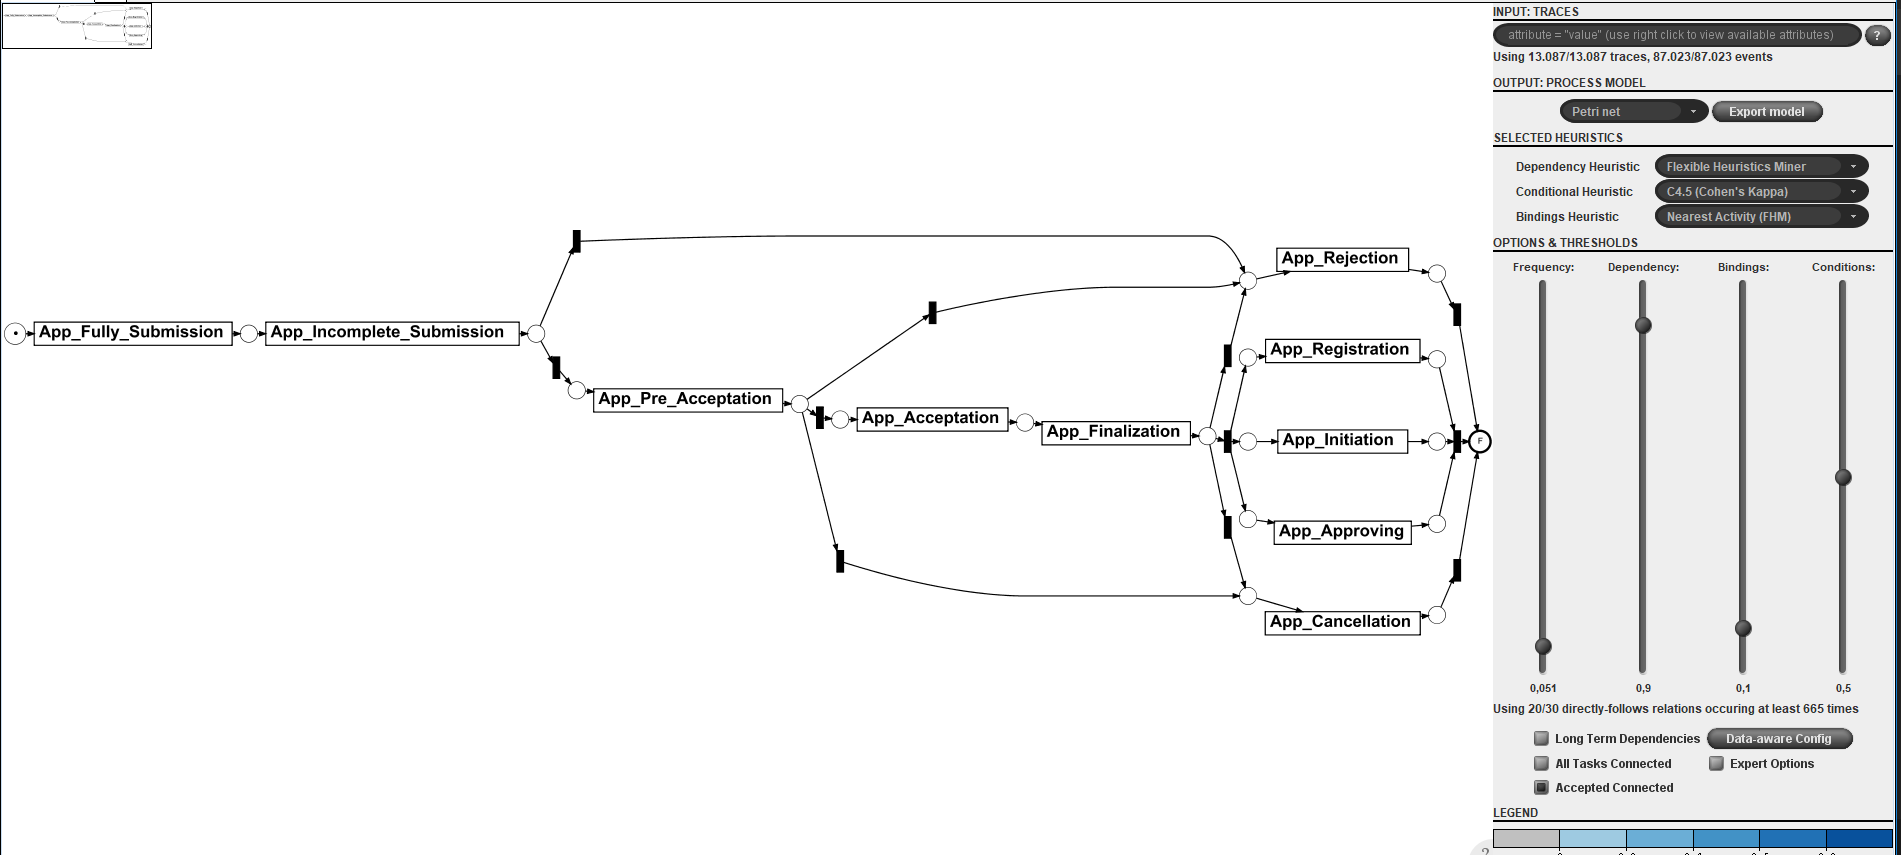
\includegraphics[width=\linewidth]{App_DirectlyFollowedFreq0-051.PNG}
  \caption{Directly followed graph 0.051 frequency}
  \label{fig:APP_DFG0-51}
\end{subfigure}
\begin{subfigure}{.49\textwidth}
  \centering
  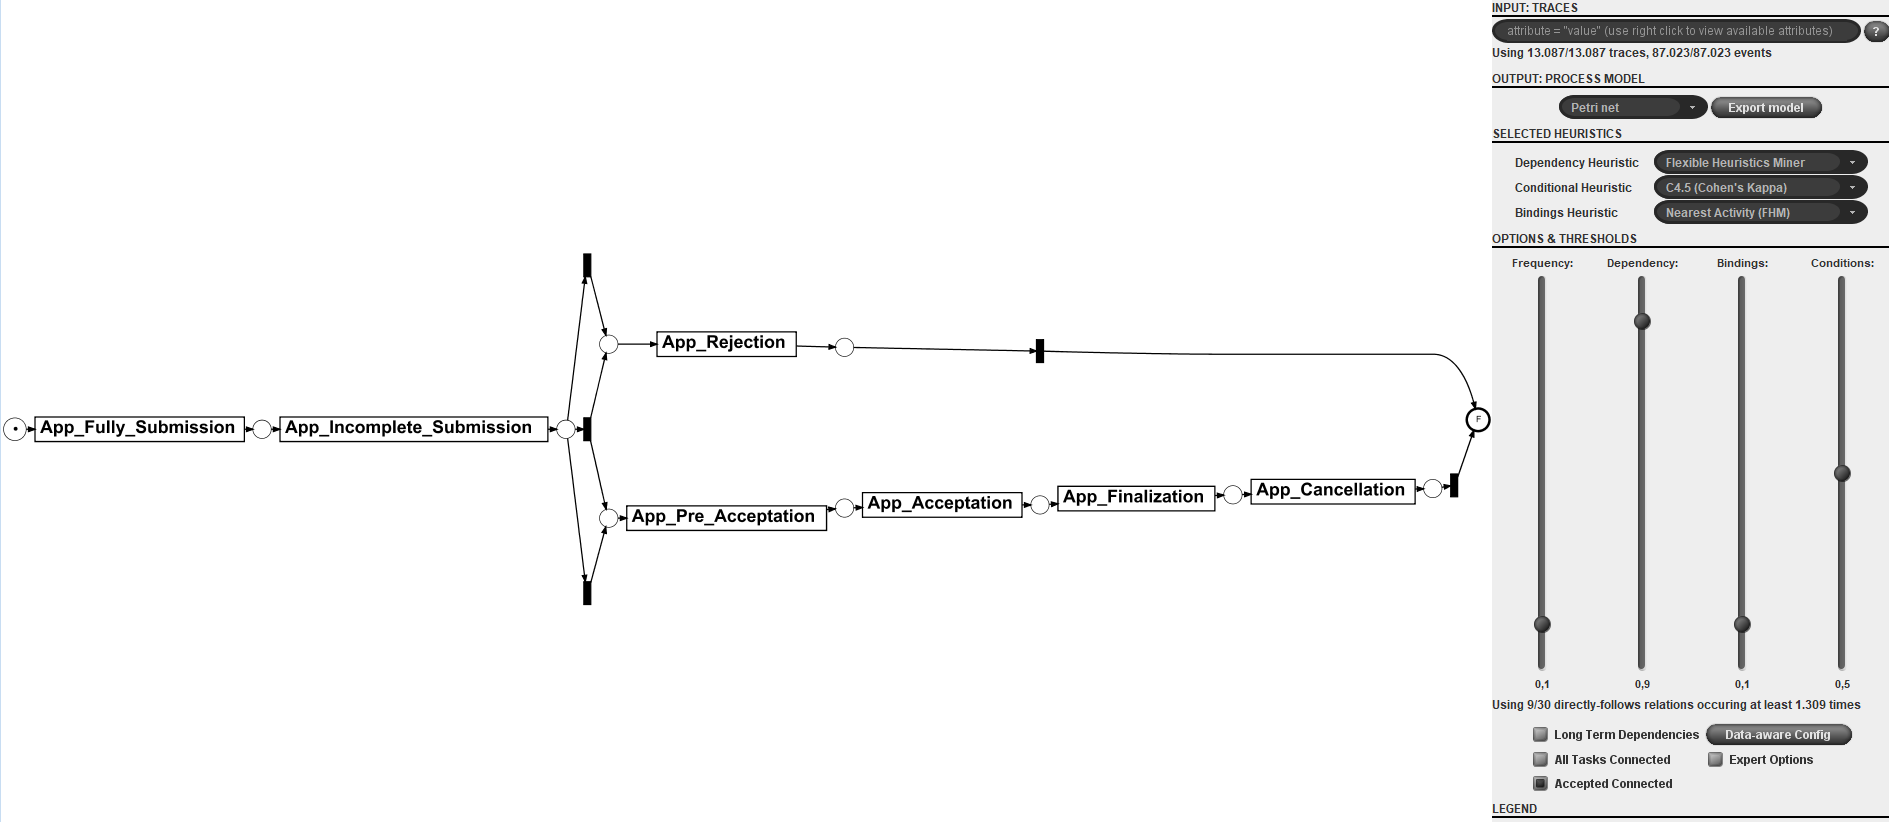
\includegraphics[width=\linewidth]{App_DirectlyFollowedFreq0-1.PNG}
  \caption{Directly followed graph 0.1 frequency}
  \label{fig:APP_DFG0-1}
\end{subfigure}
\begin{subfigure}{.49\textwidth}
  \centering
  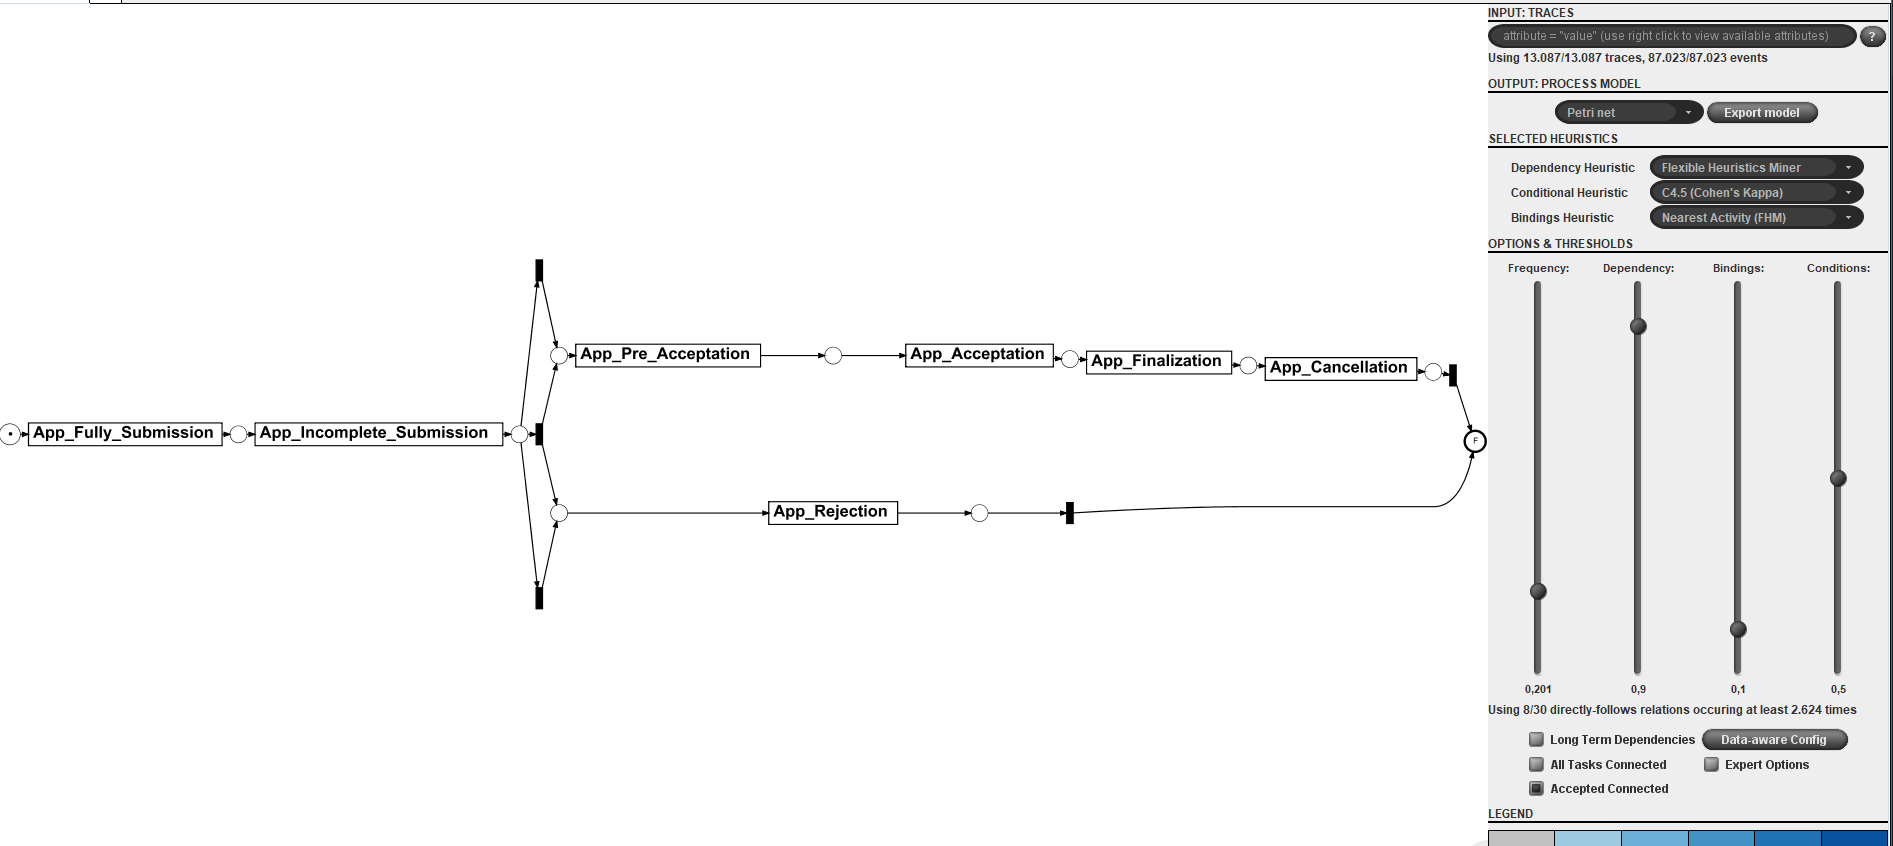
\includegraphics[width=\linewidth]{App_DirectlyFollowedFreq0-2.PNG}
  \caption{Directly followed graph 0.2 frequency}
  \label{fig:APP_DFG0-2}
\end{subfigure}
\caption{Considered directly followed graphs}
\label{fig:App_Direct}
\end{figure}

The first try I choose the frequency 0.1 and had a look at the directly followed graph. I also checked 0.2 and 0.51. For comparsion in the end I checked also the original directly followed graph. My first choice was the directly followed graph with 0.1 as threhold for frequency, because it was a simple model that still tells us a lot about the main process. In figure \ref{fig:App_Direct} the 4 considered directly followed graphs can be seen. Obviously the original graph does not fullfill the criterium of simplicity and also the graph with frequency 0.051 still looks not as simpel as I would like.

\begin{figure}[h]
\centering
\begin{subfigure}{.3\textwidth}
  \centering
  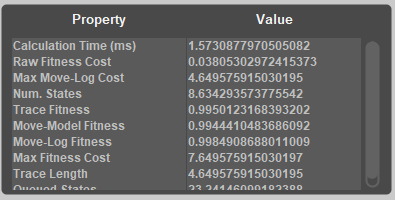
\includegraphics[width=\linewidth]{App_Conformance0-051.PNG}
  \caption{Conformance for 0.051 frequency}
  \label{fig:APP_Conf0-051}
\end{subfigure}%
\begin{subfigure}{.3\textwidth}
  \centering
  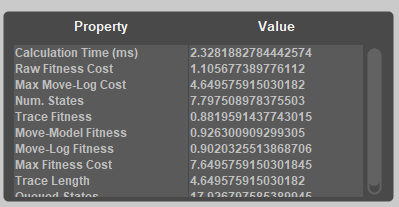
\includegraphics[width=\linewidth]{App_Conformance0-1.PNG}
  \caption{Conformance 0.1}
  \label{fig:APP_Conf0-1}
\end{subfigure}
\begin{subfigure}{.3\textwidth}
  \centering
  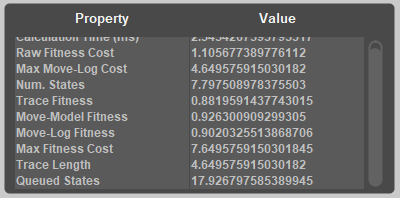
\includegraphics[width=\linewidth]{App_Conformance0-2.PNG}
  \caption{Conformance for 0.2 frequency}
  \label{fig:APP_Conf0-2}
\end{subfigure}
\caption{Conformance checking}
\label{fig:App_Conf}
\end{figure}

In the next step I checked the conformance of the corresponding petri net, which I exported from the Interactive Data-aware Heuristic Miner, by combining the data and the petri net for the conformance checking with the Replay tool for Conformance checking. 
The results in \ref{fig:App_Conf} showed me, that the model with 0.2 also has the same conformance than 0.1, what is not surprising, because they have the same petri-net. Based on this and the fact, that the conformance of 0.1 filtered is still not so bad I considered 0.051 and 0.1 for the precision check.

Applying the Multi-perspective Process Explorer and choosing "show precision mode".

\begin{figure}[h]
\centering
\begin{subfigure}{.49\textwidth}
  \centering
  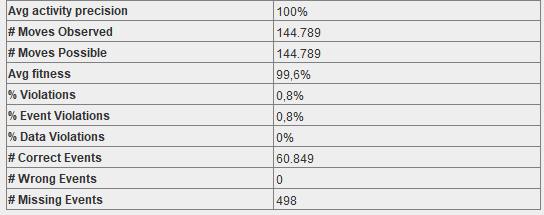
\includegraphics[width=\linewidth]{App_Precision0-051.PNG}
  \caption{Precision for 0.051 as frequency}
  \label{fig:APP_Prec0-051}
\end{subfigure}%
\begin{subfigure}{.49\textwidth}
  \centering
  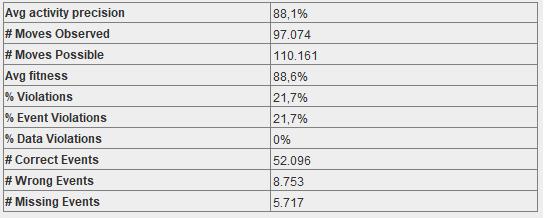
\includegraphics[width=\linewidth]{App_Precision0-1.PNG}
  \caption{Precision for 0.1 as frequency}
  \label{fig:APP_Prec0-1}
\end{subfigure}
\caption{Precision checking}
\label{fig:App_Prec}
\end{figure}

%0.07
Checking the precision, \ref{fig:App_Prec}, and combine it with the results before, I came to the conclusion, that 0.1 is not good enough as model and 0.051 is good enough, but too complicated. Starting by this I again tried different frequency filters outgoing by 0.075 to find a model, which has a similar simplicity than the 0.1 frequency model, but a better conformance and precision. And already the frequency filtering 0.076 gives me the wished result.

\begin{figure}[h]
\centering
\begin{subfigure}{.49\textwidth}
  \centering
  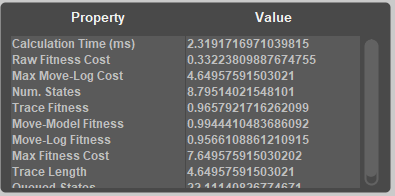
\includegraphics[width=\linewidth]{App_Conformance0-076.PNG}
  \caption{Conformance}
  \label{fig:APP_Conf0-076}
\end{subfigure}
\begin{subfigure}{.49\textwidth}
  \centering
  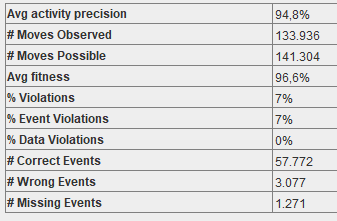
\includegraphics[width=\linewidth]{App_Precision0-076.PNG}
  \caption{Precision}
  \label{fig:APP_Prec0-076}
\end{subfigure}
\begin{subfigure}{\textwidth}
  \centering
  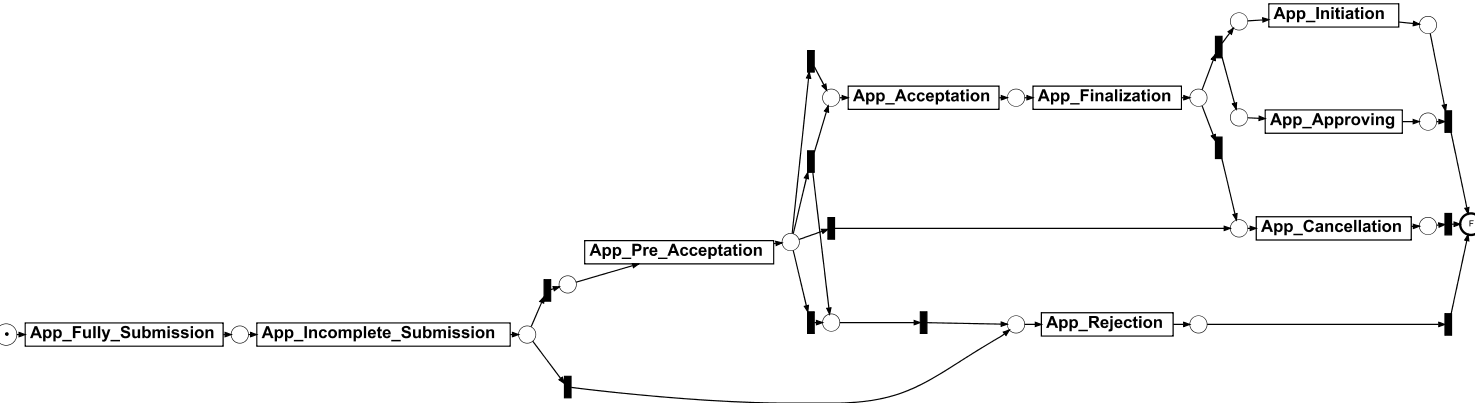
\includegraphics[width=\linewidth]{App_DirectlyFollowedFreq0-076.PNG}
  \caption{Directly followed graph}
  \label{fig:APP_DF0-076}
\end{subfigure}%
\caption{Frequency 0.076}
\label{fig:App_Prec}
\end{figure}

This model has a good simplicity, but still has a path fitness of 96.58\% and precision of 94.8\%, so it is still pretty good. Overall I so decided to choose the 0.076 frequency model for the application's lifecycle.


\subsection*{The model of the proposal's lifecycle }

Applying the same steps on the proposal lifecycle gave me first 4 models to have a closer look at.


\begin{figure}[h]
\centering
\begin{subfigure}{.49\textwidth}
  \centering
  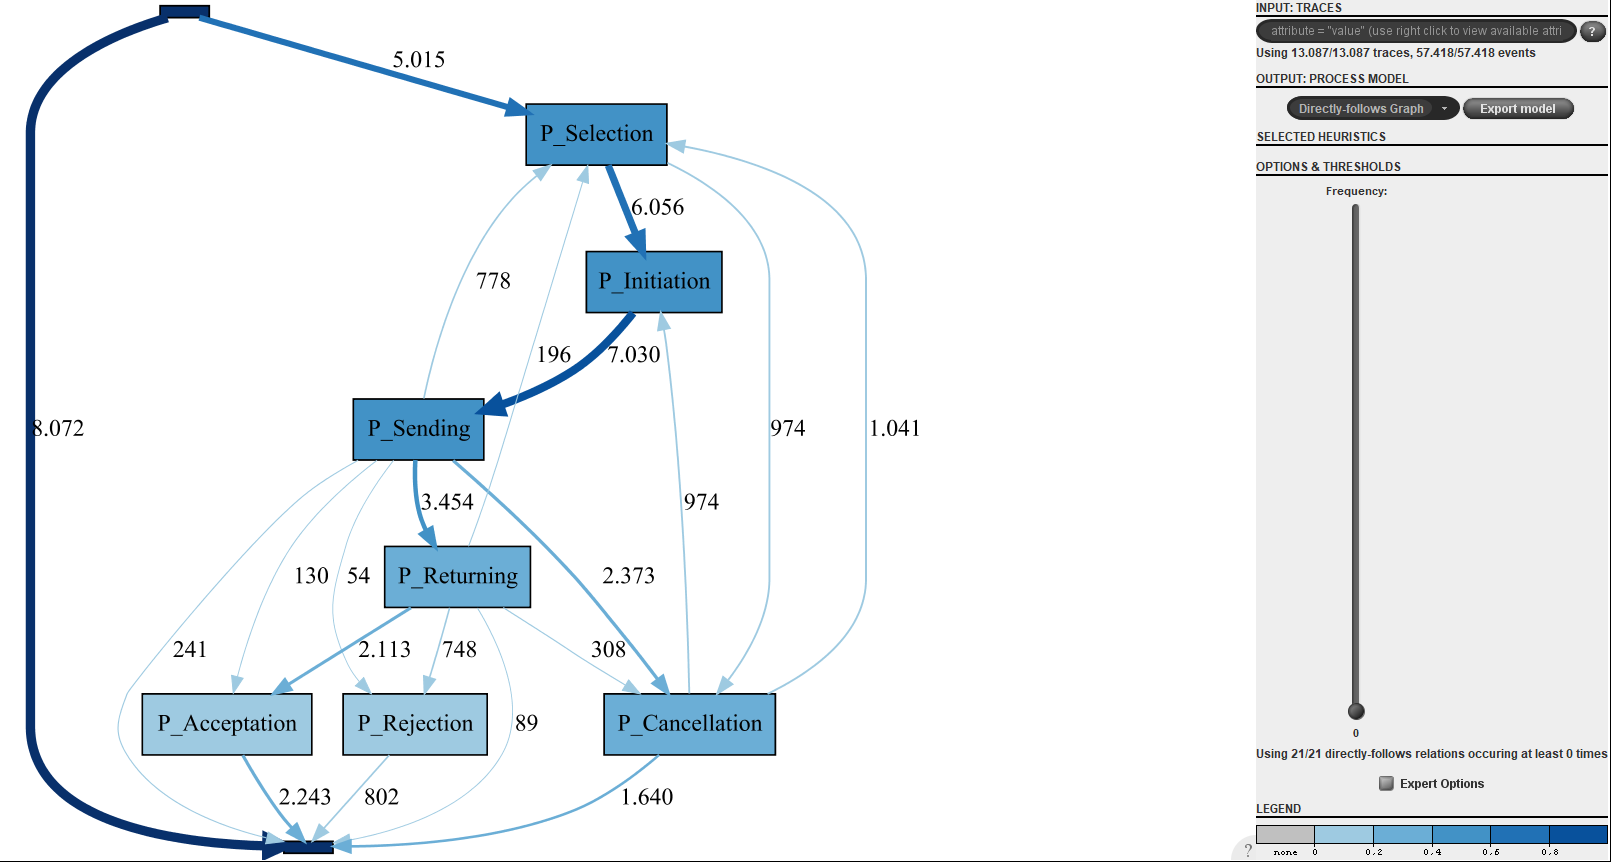
\includegraphics[width=\linewidth]{P_DirectlyFollowedFreq0.PNG}
  \caption{Directly followed graph without frequency filtering}
  \label{fig:P_DFG0}
\end{subfigure}%
\begin{subfigure}{.49\textwidth}
  \centering
  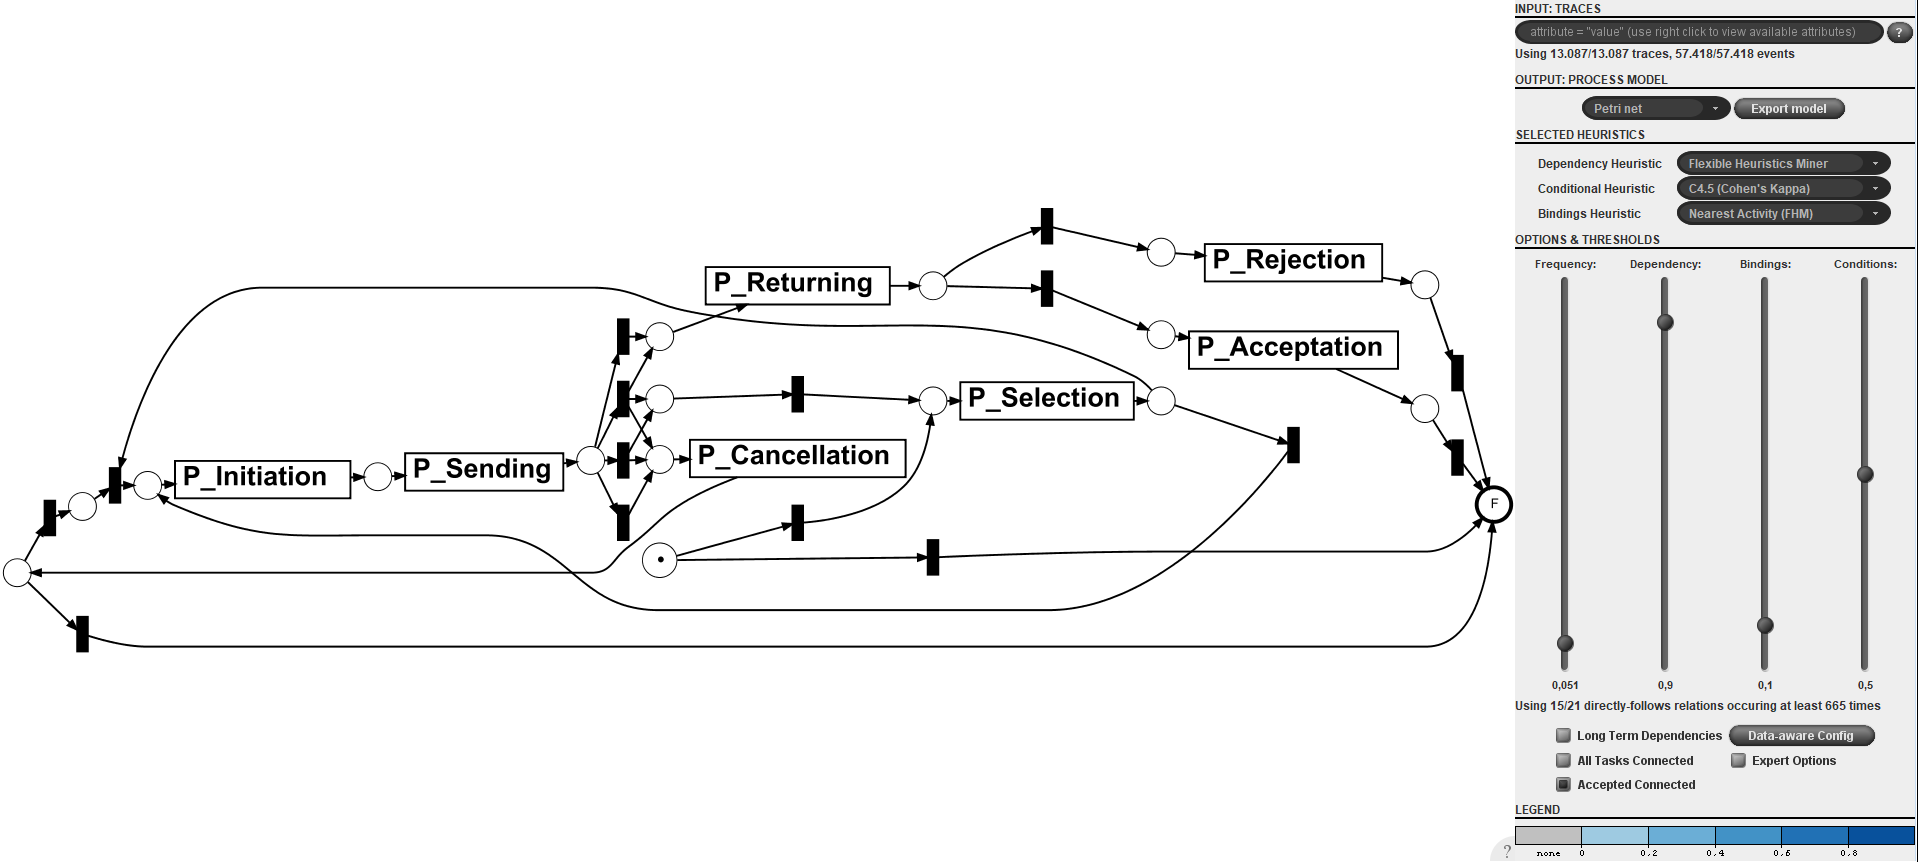
\includegraphics[width=\linewidth]{P_DirectlyFollowedFreq0-051.PNG}
  \caption{Directly followed graph 0.051 frequency}
  \label{fig:P_DFG0-051}
\end{subfigure}
\begin{subfigure}{.49\textwidth}
  \centering
  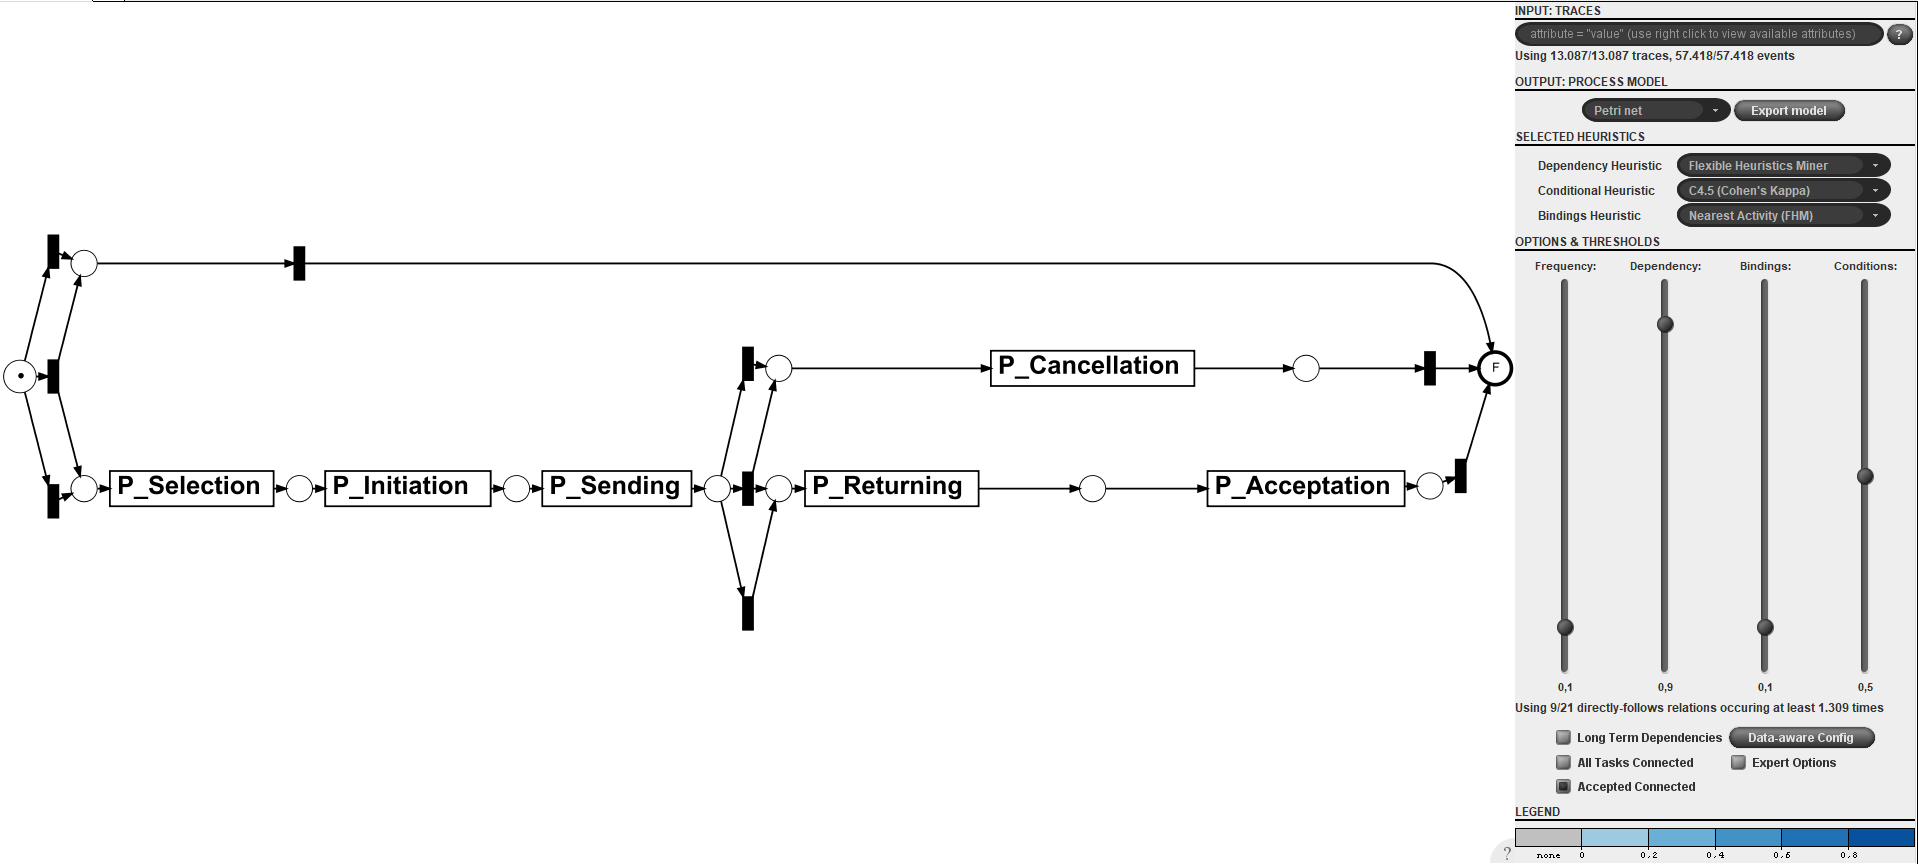
\includegraphics[width=\linewidth]{P_DirectlyFollowedFreq0-1.PNG}
  \caption{Directly followed graph 0.1 frequency}
  \label{fig:P_DFG0-1}
\end{subfigure}
\begin{subfigure}{.49\textwidth}
  \centering
  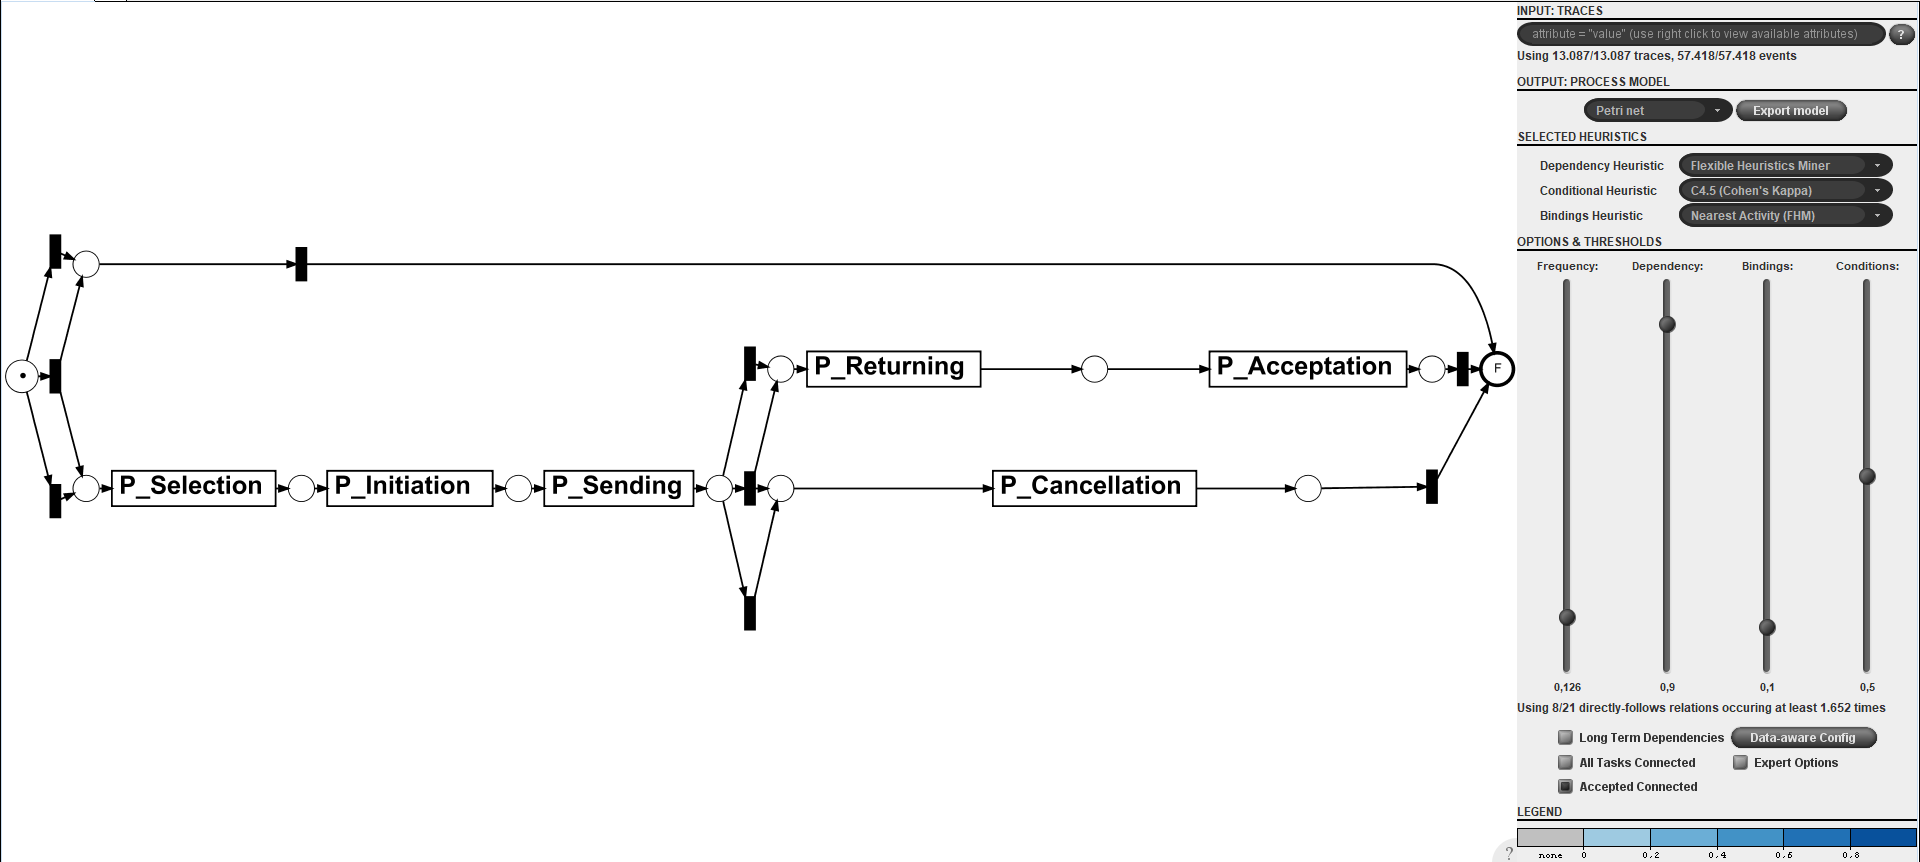
\includegraphics[width=\linewidth]{P_DirectlyFollowedFreq0-126.PNG}
  \caption{Directly followed graph 0.126 frequency}
  \label{fig:P_DFG0-126}
\end{subfigure}
\caption{Considered directly followed graphs}
\label{fig:P_Direct}
\end{figure}

Because of simplicity I first checked the conformance and precision just for 0.051 and 0.1 frequency filtering. 

\begin{figure}[h]
\centering
\begin{subfigure}{.5\textwidth}
  \centering
  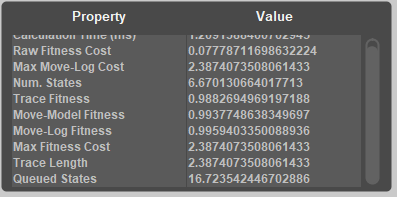
\includegraphics[width=\linewidth]{P_Conformance0-051.PNG}
  \caption{Conformance for 0.051 frequency}
  \label{fig:P_Conf0-051}
\end{subfigure}%
\begin{subfigure}{.5\textwidth}
  \centering
  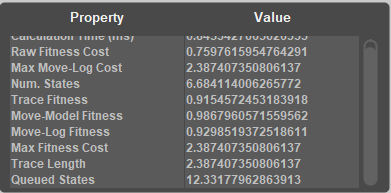
\includegraphics[width=\linewidth]{P_Conformance0-1.PNG}
  \caption{Conformance 0.1}
  \label{fig:P_Conf0-1}
\end{subfigure}
\begin{subfigure}{.49\textwidth}
  \centering
  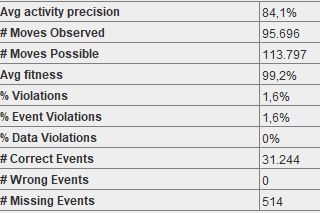
\includegraphics[width=\linewidth]{P_Precision0-051.PNG}
  \caption{Precision for 0.051 as frequency}
  \label{fig:P_Prec0-051}
\end{subfigure}%
\begin{subfigure}{.49\textwidth}
  \centering
  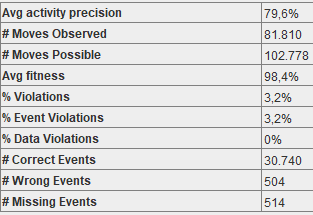
\includegraphics[width=\linewidth]{P_Precision0-1.PNG}
  \caption{Precision for 0.1 as frequency}
  \label{fig:P_Prec0-1}
\end{subfigure}
\caption{Conformance and precision checking}
\label{fig:P_ConfPrec}
\end{figure}


Having a look at the different conformance and precision outcomes \ref{fig:P_ConfPrec}, I decided, that the 0.1 frequency model is not good enough, but wanted to check, if there is a model better or in simplicity or in performance for the 0.051 model. The models best for simplicity fitting had 0.08 frequency or 0.025.

\begin{figure}[h]
\centering
\begin{subfigure}{.49\textwidth}
  \centering
  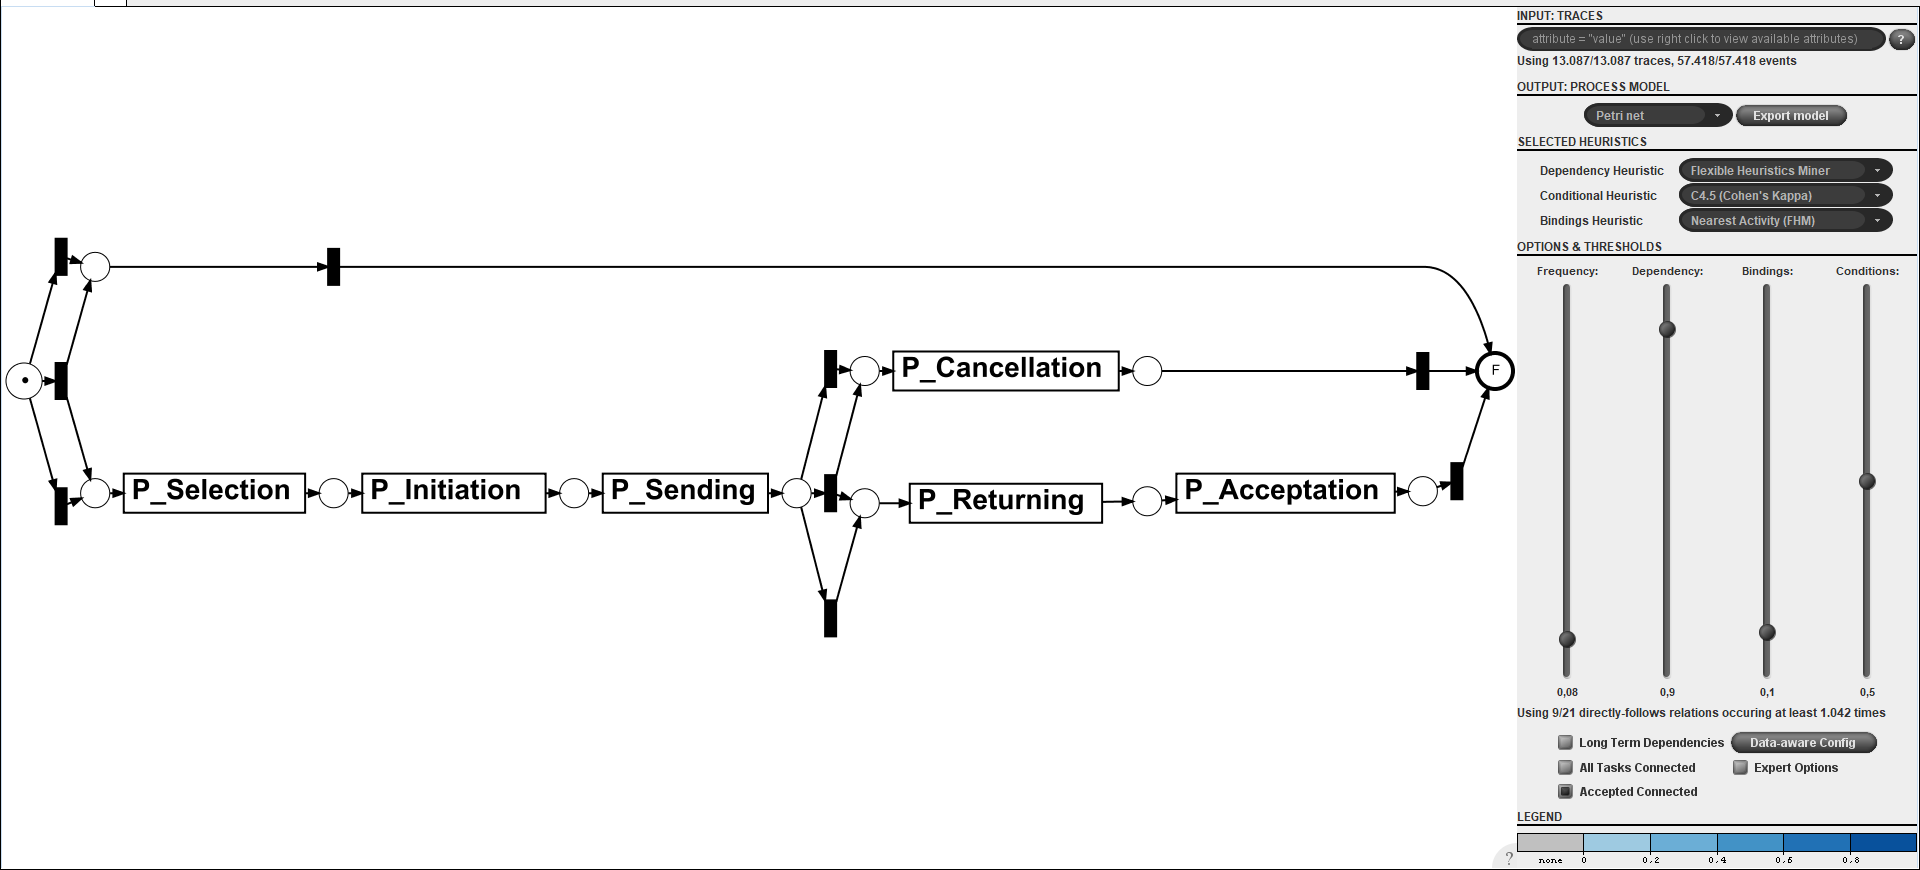
\includegraphics[width=\linewidth]{P_DirectlyFollowedFreq0-08.PNG}
  \caption{Directly followed graph 0.08 frequency}
  \label{fig:P_DFG0-08}
\end{subfigure}
\begin{subfigure}{.49\textwidth}
  \centering
  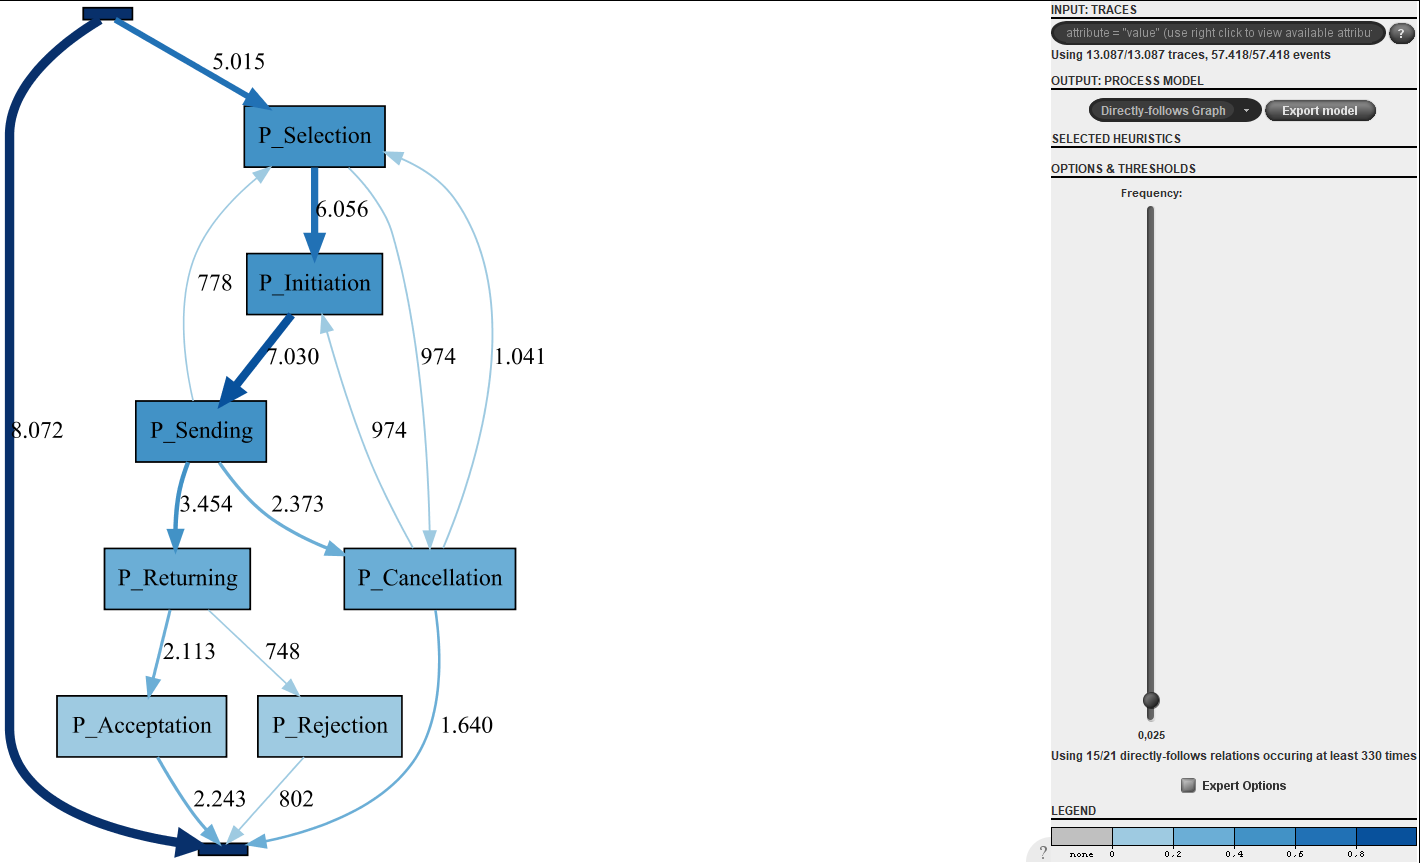
\includegraphics[width=\linewidth]{P_DirectlyFollowedFreq0-025.PNG}
  \caption{Directly followed graph 0.025 frequency}
  \label{fig:P_DFG0-025}
\end{subfigure}%
\begin{subfigure}{.5\textwidth}
  \centering
  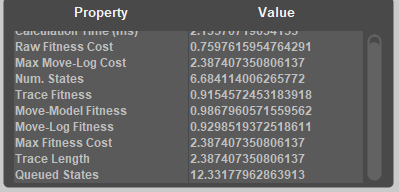
\includegraphics[width=\linewidth]{P_Conformance0-08.PNG}
  \caption{Conformance for 0.08 frequency}
  \label{fig:P_Conf0-08}
\end{subfigure}%
\begin{subfigure}{.5\textwidth}
  \centering
  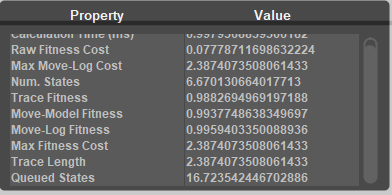
\includegraphics[width=\linewidth]{P_Conformance0-025.PNG}
  \caption{Conformance 0.025}
  \label{fig:P_Conf0-025}
\end{subfigure}
\begin{subfigure}{.49\textwidth}
  \centering
  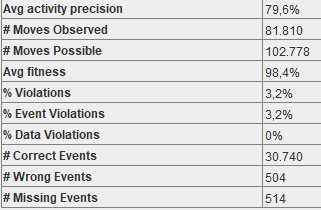
\includegraphics[width=\linewidth]{P_Precision0-08.PNG}
  \caption{Precision for 0.08 as frequency}
  \label{fig:P_Prec0-08}
\end{subfigure}%
\begin{subfigure}{.49\textwidth}
  \centering
  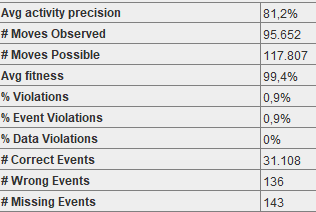
\includegraphics[width=\linewidth]{P_Precision0-025.PNG}
  \caption{Precision for 0.025 as frequency}
  \label{fig:P_Prec0-025}
\end{subfigure}
\caption{Directly followeg graphs, conformance and precision}
\label{fig:P_Direct2}
\end{figure}

After checking all results in \ref{fig:P_Direct2} I had to choose.
This was a hard decision, but I chose simplicity over the precision and picked the model with 0.025. The fitness is above 90\% and precision is also okay. Lower frequency threshold just makes the model to complicated.

\subsection*{Combinded Model}
%Models that combine these two models into one showing the lifecycle of the application and the proposal together. Due to the high variability, you should discover one different model for each possible outcome, namely whether the application is finally rejected, cancelled or approved. 
First I filtered the data 3 times to have a dataset with all p


\subsection*{C-net of the proposal process}
%Analyze the C-net of the proposal process and explain it. 

\subsection*{Own Petri net of the proposal process}
%Based on your analysis, create a Petri net of the proposal process by your own. For example, do not consider infrequent paths and also outlier behaviors. 

\subsection*{Analysis of the performance of Application and work process}
%Analyze the performance of Application and work process. What are the bottlenecks? What are your recommendations to the company to increase the performance of the process? 